\chapter{Soluzione Proposta}\label{chap:soluzioneproposta}

\section{Introduzione} \label{sec:solIntroduction}

L'estrazione dei dati dalla blockchain di Bitcoin ha richiesto un analisi preliminare della tecnologia ed in particolare sul modo in cui vengono serializzati i dati dal client; questa prima analisi ha permesso di osservare la rapida crescita dello spazio richiesto della blockchain, rappresentata dalla Figura \ref{fig:dimensionBlockchain}.

{\vspace{15pt}
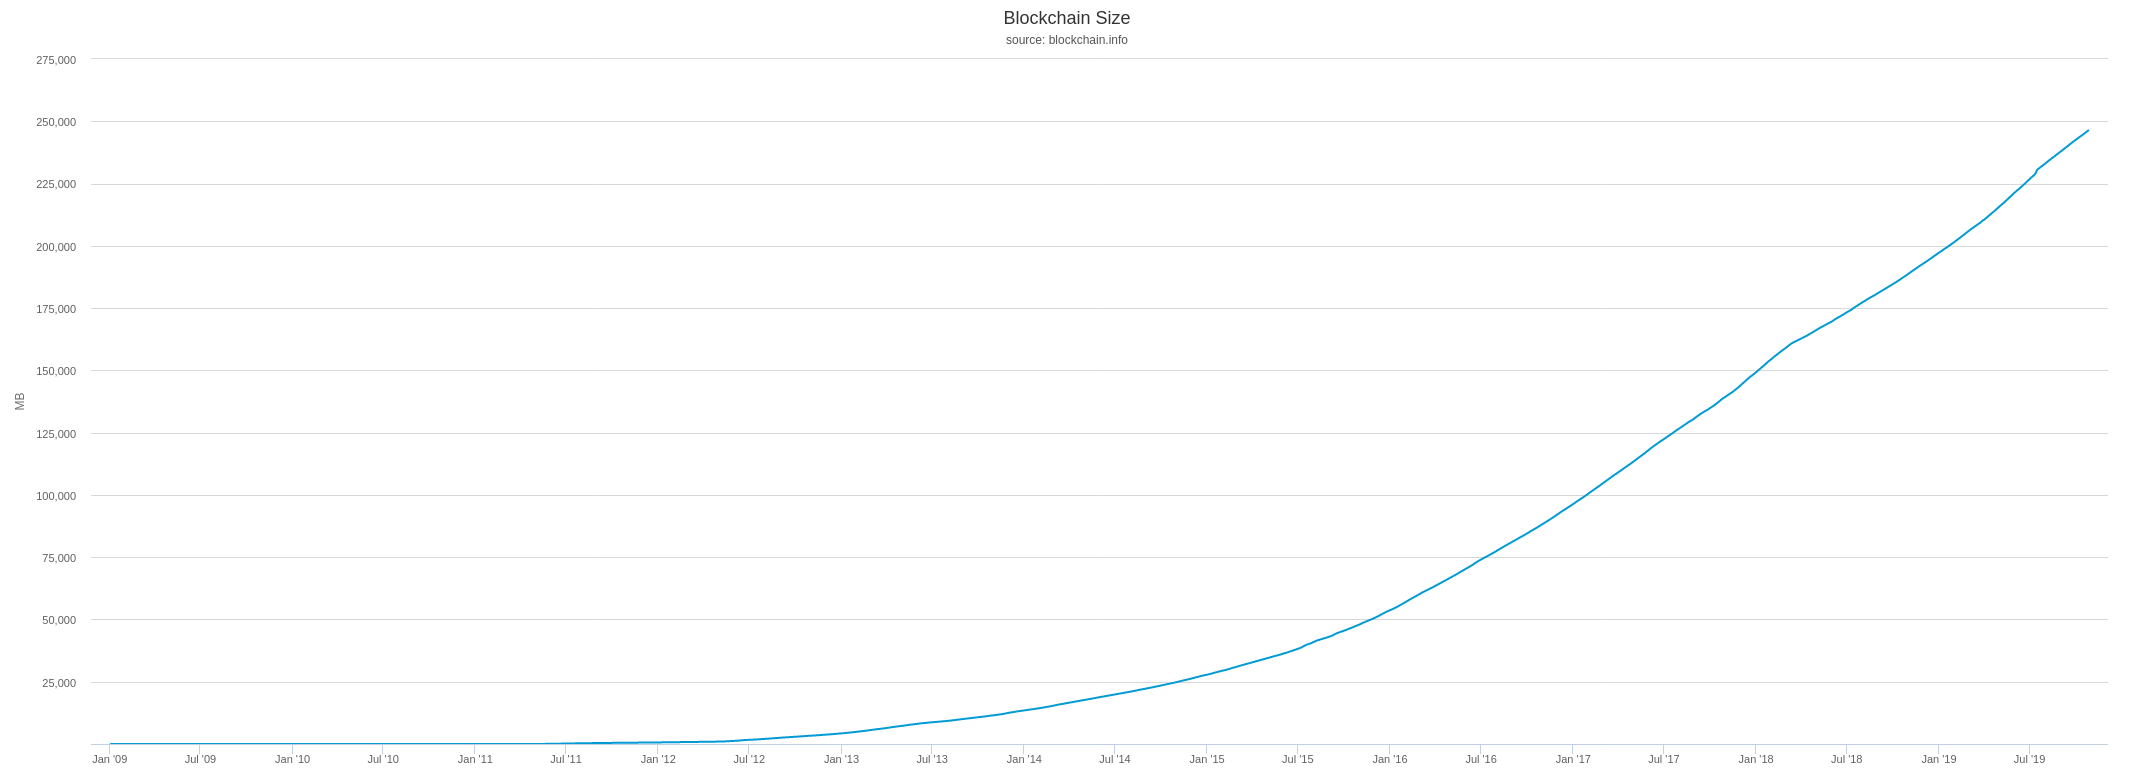
\includegraphics[scale=0.18]{images/blockchain-size.png}
\captionof{figure}{Crescita della dimensione della blockchain di Bitcoin nel tempo.\label{fig:dimensionBlockchain}}
\vspace{10pt}
\par}

La rapida crescita della blockchain porta alle seguenti problematiche:

\begin{itemize}
  \item L'estrazione dei dati dalla blockchain di Bitcoin richiede un software scalabile per permettere in qualsiasi condizione di utilizzo l'estrazione dei dati.
  \item L'organizzazione dei dati estratti della blockchain deve essere versatile per consentire analisi differenti, in modo tale da non richiedere una seconda scansione a seconda del tipo di analisi da effettuare.
\end{itemize}

\section{SpyCBlock} \label{sec:spycblock}

SpyCBlock rappresenta la soluzione proposta per l'estrazione di dati dalla blockchain di Bitcoin in modo scalabile. Attraverso SpyCBlock viene effettua la creazione dei due principali grafi per l'analisi forense; SpyCBlock, inoltre, produce in formato JSON (JavaScript Object Notation) una deserializzazione completa della blockchain, arricchita con informazioni addizionali; infatti, come descritto nel Capitolo \ref{chap:bitcoin}, i blocchi e le transazioni contengono solo gli identificativi dei loro predecessori, il che costringe il parser in fase di deserializzazione a ricostruire l'hash della transazione e del rispettivo blocco preso in analisi; questo è stato reso possibile dalla libreria \say{Bitcoin-Cryptography-Library} descritta nel Capitolo \ref{sec:cryptographyBitcoinLib}.\\
SpyCBlock rappresenta un prototipo di un software di analisi accademico, sviluppato interamente in C++ e risiede su Github sotto licenza Apache License 2.0. Esso è l'implementazione di un parser delle informazioni serializzate dal nodo Bitcoin e utilizza le librerie di Bitcoin-core, descritte nella Sezione \ref{sec:bitcoinCoreLib}.\\
Il software è stato implementato utilizzando una metodologia agile; infatti lo sviluppo di SpyCBlock e lo studio della tecnologia Bitcoin sono avvenute in parallelo. Questo ha permesso di convalidare tutte le nozioni studiate sulla tecnologia, basando l'intero ciclo di sviluppo sulla produzione di test di unità (10 batterie di test, per un totale di 60 test di unità).\\
I dati decodificati del singolo blocco vengono verificati all'interno dei test di unità utilizzando dati prodotti attraverso l'utilizzo di altri parser, come Blocktools \cite{parser:blocktools}, e attraverso i dati esposti dagli explorer, come Explora \cite{blockstream:esplora} e Blockchain explorer \cite{blockchain:explorer}.\\
Inoltre il parser è costituito da un sottomodulo per consentire la costruzione del grafo di address, utilizzando il nodo Bitcoin-core per effettuare la decodifica degli script.

\section{SpyCBlockRPC} \label{sec:spycblockrpc}

SpyCBlockRPC è un sottomodulo di SpyCBlock descritto nella Sezione \ref{sec:spycblock}; esso viene sviluppato in C++ e risiede su Github sotto licenza Apache License 2.0.\\
SpyCBlockRPC rappresenta l'implementazione di un wrapper della libreria bitcoin-api-cpp descritta nella Sezione \ref{sec:bitcoinApiLib} che consente di effettuare interi casi d'uso costituiti da più comandi RPC di Bitcoin-core.
L'utilizzo di questo sottomodulo permette al parser di rimanere disaccoppiato dalla libreria bitcoin-cpp-api e dal framework RPC; inoltre il sottomodulo fornisce un'interfaccia comune per la serializzazione di qualsiasi tipo di grafo che si voglia costruire usando le informazioni della blockchain.\\
SpyCBlock utilizza l'interfaccia comune offerta da SpyCBlockRPC per implementare la serializzazione del grafo di transazioni ed inoltre utilizza l'implementazione offerta dal sottomodulo SpyCBlockRPC per serializzare il grafo degli address.

\section{Serializzazione della blockchain in formato JSON} \label{sec:spycblock}

Prima di effettuare la creazione dei grafi, descritti nelle sezioni successive, abbiamo dovuto affrontare varie problematiche che si sono presentate durante la fase di decodifica delle informazioni. Infatti, l'aggiornamento al Segregated Witness (descritto nella Sezione \ref{sec:transazionibitcoincore}) ha introdotto alcune modifiche anche nel modo in cui viene serializzata una transazione; questo costringe il parser a utilizzare, a seconda del tipo di transazione, metodi diversi di deserializzazione.
L'aggiornamento al Segregated Witness ha introdotto tre nuove informazioni all'interno delle transazioni, che sono:
\begin{itemize}
  \item La proprietà flag.
  \item La proprietà Marker.
  \item Se le due proprietà precedenti sono rispettivamente 0 e 1, allora all'interno della transazione esisterà una lista di Script Witness, descritti nella Sezione \ref{sec:transazionibitcoincore}, che vengono denominati \say{TransactionWitness}.
\end{itemize}

Il Frammento di codice descritto nell'Appendice \ref{sec:decodeTransactionCode} rappresenta il codice con cui è possibile deserializzare una transazione dopo l'aggiornamento al Segregated Witness (viene usato Python per brevità).\\
I problemi relativi alla deserializzazione dei dati, combinati con la grande quantità di dati da deserializzare\footnote{In data {\today} la dimensione della blockchain di Bitcoin è pari a 249 Gb.}, hanno richiesto la progettazione di un metodo di testing automatico sull'intera blockchain oppure su un parte specifica.
Questo ha richiesto di convertire le informazioni deserializzate dal parser in un formato universale per eseguire l'elaborazione di queste informazioni con qualsiasi linguaggio.\\
Il formato file utilizzato per la codifica delle informazioni è il formato JSON (JavaScript Object Notation) e la libreria RapidJSON descritta nella Sezione \ref{sec:rapidjsonLib} ha reso possibile la serializzazione delle informazioni lette dal parser in maniera streaming: ogni blocco decodificato viene serializzato in JSON immediatamente con la conseguenza di un utilizzo di memoria RAM irrisorio.\\
L'adozione del formato JSON per l'organizzazione dei dati ha portato i seguenti benefici:
\begin{itemize}
  \item I dati serializzati in JSON possono essere testati in maniera automatizzata attraverso l'uso di API esterne oppure attraverso il framework RPC di Bitcoin-core descritto nella Sezione \ref{sec:jsonrpchttp}.
  \item I dati serializzati in JSON possono essere testati a vari livelli di precisione. A titolo di esempio, un eventuale errore di deserializzazione in un determinato punto della blockchain può essere individuato facilmente e osservato attraverso il suo corrispettivo in formato JSON.
  Questo evita l'uso del debugger per errori introdotti in fase di sviluppo dal programmatore, perché essi sono facilmente individuabili se i dati sono convertiti in un formato comprensibile per l'uomo.
  \item La rappresentazione JSON dell'intera blockchain offre anche la possibilità di eseguire ulteriori tipi di analisi all'interno della blockchain di Bitcoin; ad esempio attraverso l'utilizzo di una semplice applicazione di analisi descritta nella Sezione \ref{sec:solDemo}, è possibile sfruttare i dati in formato JSON per un analisi sui tipi di script utilizzati all'interno della blockchain.
  In Figura \ref{fig:chartOPRETURN} viene riportato un grafico che rappresenta l'utilizzo estensivo dell'operatore OP\_RETURN (descritto nella Sezione \ref{sub:sectionNUllaDataScript}) e quindi l'utilizzo della blockchain di Bitcoin per l'archiviazione di dati.
\end{itemize}

{\centering
\vspace{15pt}
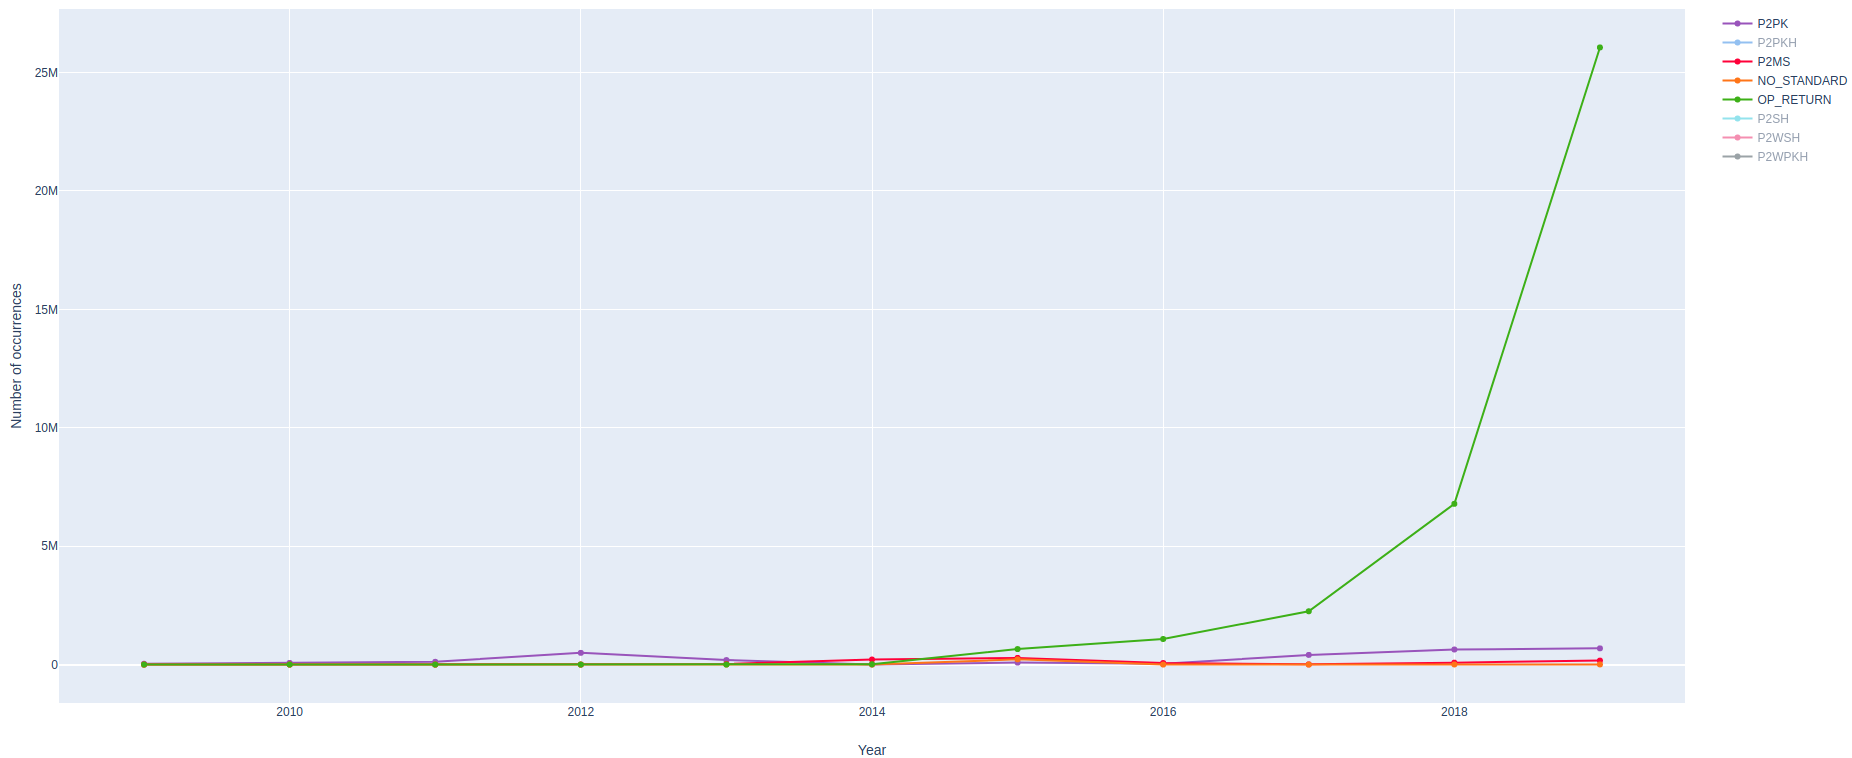
\includegraphics[scale=0.25]{images/OP_RETUTN_chart.png}
\captionof{figure}{Frammento di grafico estrapolato dall'applicazione della Sezione \ref{sec:AnalyticsPyBlock} dove viene rappresentato l'utilizzo del operatore OP\_RETURN all'interno degli script di blocco.\label{fig:chartOPRETURN}}
\vspace{10pt}
\par}


\section{Grafo delle transazioni} \label{sec:solGraphTX}

Dopo un accurata convalida dei dati deserializzati dal parser, abbiamo eseguito una nuova iterazione all'interno del ciclo di sviluppo del software, aggiungendo all'interno del parser la possibilità di serializzare i dati letti come nodi e archi di un grafo orientato.\\
Ogni transazione, infatti, genera un arco $(u, v)$ in cui il nodo di origine $u$ rappresenta l'hash della transazione attualmente analizzata e il nodo di arrivo $v$ rappresenta l'hash della transazione precedente, contenuta all'interno del tipo di dato \say{Outpoint} nella transazione di input (illustrato nella Sezione \ref{sec:transazionibitcoincore}).\\
Come descritto nella Sezione \ref{sec:grafoDelleTransazioniProblema}, la creazione del grafo delle transazioni risulta abbastanza intuitiva, ma la struttura dati della blockchain di Bitcoin costringe il parser al calcolo dell'hash della transazione attualmente analizzata perché esso non viene incluso; per fare questo il parser riconverte in memoria i dati nel formato di serializzazione originario.
In seguito alla riconversione con l'utilizzo della libreria Bitcoin-Cryptography-Library descritta nella Sezione \ref{sec:cryptographyBitcoinLib}, viene eseguito il doppio SHA256 dei bit riguardanti le informazioni in formato esadecimale, in cui ogni tipo della struttura viene prima convertito nel formato little-endian.\\

\begin{example}

Prendiamo in considerazione la transazione coinbase del blocco di genesi\footnote{Il blocco di genesi è anche conosciuto come blocco 0 oppure blocco \emph{never mined}, i cui dati sono stati codificati da Satoshi Nakamoto all'interno del codice sorgente di Bitcoin-core. Introdurre dei nuovi dati all'interno del blocco di genesi implica la creazione di una nuova blockchain.} rappresentata nella Figura \ref{fig:txGenesisBlock}.

{\centering
\vspace{15pt}
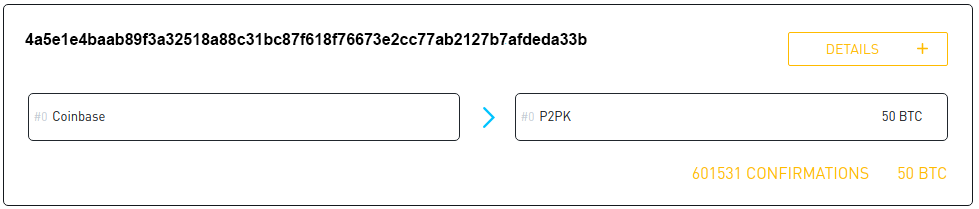
\includegraphics[scale=0.35]{images/coinbase_tx_genesis_block.png}
\captionof{figure}{Rappresentazione attraverso un'explorer \cite{blockstream:esplora} della transazione coinbase contenuta all'interno del blocco di genesi.\label{fig:txGenesisBlock}}
\vspace{10pt}
\par}

Analizzando i dati estratti dal parser possiamo notare che gli explorer non mostrano molte delle informazioni contenute all'interno delle transazioni; utilizzando invece il frammento di serializzazione JSON descritto nell'Appendice \ref{sec:genesiBlockTxJSON} in cui viene raffigurata la prima transazione nella blockchain di Bitcoin, possiamo notare tutte le informazioni realmente contenute nella struttura di una transazione.
Per effettuare il calcolo dell'hash della transazione il parser riconverte ogni tipo di dato nel formato little-endian e infine converte il valore nel corrispettivo esadecimale. La porzione di Codice \ref{code:typehexTxCpp} riporta il valore convertito con il processo descritto in precedenza.

\lstinputlisting[language=C++, label=code:typehexTxCpp, caption=Frammento di codice che rappresenta il valore esadecimale di ogni tipo di dato della transazione.]{code/coinBaseTxGenesisBlockHex.cpp}

Infine il codice in Appendice \ref{code:processBuilHashTx} riporta un test di unità del progetto SpyCBlock in cui si effettua il processo di creazione dell'hash completo.

Dopo aver ottenuto l'identificativo della transazione, il parser procede nella serializzazione della transazione come un arco $(u, v)$, aggiungendo delle informazioni addizionali all'arco, quali  l'altezza del blocco calcolato durante il parsing; quest'ultima corrisponde alla sua posizione nella catena della blockchain.
Inserendo il valore calcolato come informazione dell'arco si evita di inserire l'hash del blocco in cui risiede la transazione; questo implica un notevole risparmio di spazio delle informazioni serializzate. Inoltre, vengono inseriti anche i valori corrispondenti al numero di bitcoin spediti e il valore nLockTime.\\
La serializzazione delle informazioni avviene in streaming, cioè ogni blocco letto viene immediatamente convertito nel file contenente tutte le informazioni delle transazioni, ottenendo un formato come quello rappresentato dal Codice \ref{code:archExampleTxGrapg}.\\

\lstinputlisting[label=code:archExampleTxGrapg, caption=Informazioni della transazione in Figura \ref{fig:txGenesisBlock} decodificata nell'arco corrispondente.]{code/exampleArch.txt}

\end{example}

Attraverso la serializzazione delle transazioni con il formato appena descritto è stato possibile realizzare un applicativo web, chiamato SpyJSBlock e descritto nella Sezione \ref{sec:SpyJSBlock}, per la visualizzazione del grafo utilizzando la libreria JavaScript descritta nella Sezione \ref{sec:ngraph}. Nella Figura \ref{fig:visgraphTx} è rappresentata una porzione di grafo delle transazioni; da tale rappresentazione si può notare  l'enorme quantità di transazioni contenute in una piccola parte di blockchain (50 Mb di 249 Gb) che rende difficile il rendering di esse.
Attraverso alcuni zoom effettuati si può notare l'esistenza di piccole comunità di nodi che scambiano bitcoin; in particolare possiamo notare dallo zoom \say{B} alcuni nodi che fanno parte di transazioni M:1.

\begin{figure}
\centering
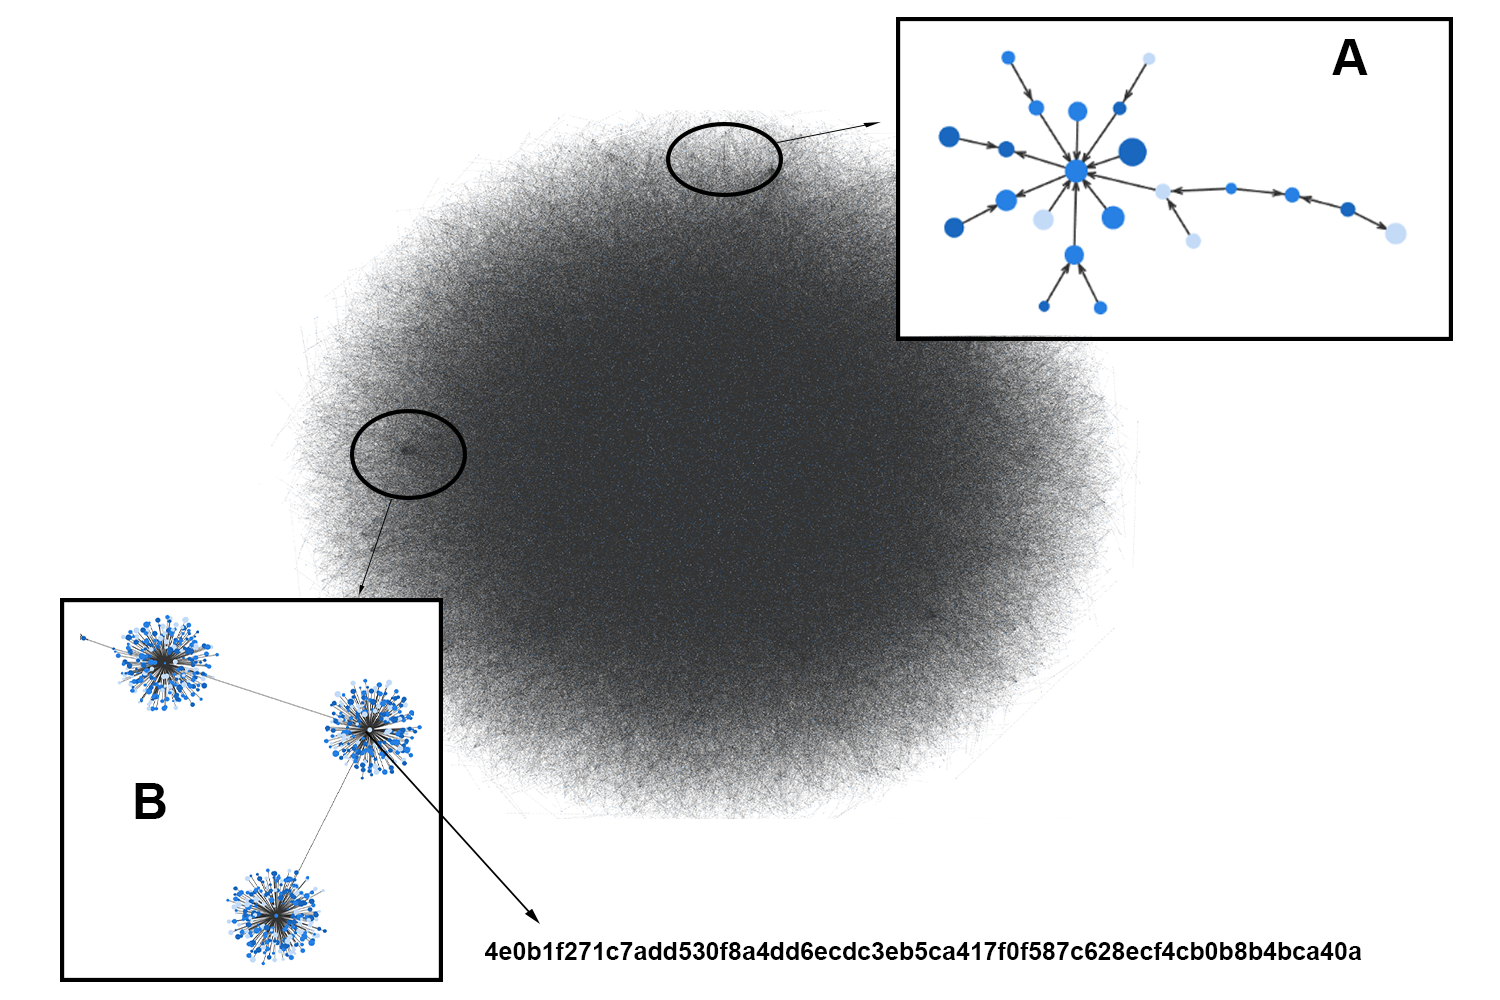
\includegraphics[scale=0.25]{images/demo/graph_tx_demo_presentation.png}
\caption{Porzione di grafo delle transazioni visualizzata attraverso SpyJSBlock.}
\label{fig:visgraphTx}
\end{figure}

\begin{example}
Consideriamo lo zoom \say{B} della Figura \ref{fig:visgraphTx}. Possiamo notare 3 comunità di nodi, in cui solo uno di esso spedisce bitcoin ad un altra comunità.\\
  Prendendo in considerazione il nodo con  identificativo di transazione \say{4e0b1f\-271c7add\-530f8a4dd6e\-cdc3eb5ca41\-7f0f587c6\-28ecf4cb0\-b8b4b\-ca40a}, si può notare attraverso l'uso di uno explorer che la transazione contiene 236 transazioni di input e 1 transazione di output, questo potrebbe indicare che il wallet abbia raggruppato tutte le transazioni su un unico address.
\end{example}

La blockchain di bitcoin serializza i blocchi all'interno di file chiamati \say{blk00000.dat} dove \say{00000} rappresenta l'indice dei file; Bitcoin-core stabilisce degli standard di dimensione per i file, pari a circa 100 Mb per ogni file.\\
SpyCBlock effettua la serializzazione 1 a 1, cioè per ogni file \say{blk0000.dat} produce un file con le informazioni in un specifico formato ad esempio \say{blk00000.json}; questo dà la possibilità di far evolvere facilmente il parser verso un' implementazione parallela e/o distribuita.

\section{Grafo degli address} \label{sec:solGraphAddress}

Dopo avere implementato la  costruzione del grafo delle transazioni, ci siamo concentrati sulla costruzione del grafo degli address. Come descritto nella Sezione \ref{sec:grafoDegliAddressProblema}, la costruzione di tale grafo introduce alcune problematiche che obbligano a rivedere il modo in cui si ricavano i dati durante il parsing delle informazioni.\\
Gli address sono infatti contenuti all'interno dello script di blocco di una transazione, come illustrato nelle Sezioni \ref{sec:bitcoinScriptBitcoin} e \ref{sec:bitcoinScriptBitcoinCore}, mentre lo script di sblocco contiene solo le informazioni riguardanti le condizioni per cui un UTXO può essere sbloccato, non possedendo nessun riferimento dell'indirizzo di origine.
Per accedere allo script di blocco della precedente transazione, il cui identificativo (hash) risiede all'interno della transazione di input, appartenente alla transazione attualmente analizzata, bisogna memorizzare la cronologia delle transazioni decodificate e ricostruire un meccanismo per la gestione degl'UTXO, simile al meccanismo usato da Bitcoin-core: fornire un metodo di memorizzazione, che consente di prelevare una transazione precedentemente analizzata con costo $O(1)$ oppure con un costo logaritmico $O(N log(N))$.\\
Al momento della stesura del documento, il parser non possiede nessun meccanismo di analisi degli script; essi con il passare del tempo sono diventati molto complessi e, come illustrato nella Sezione \ref{sec:noStrandardScript}, sono stati   introdotti metalinguaggi (come miniscript) per facilitare la scrittura di script \say{no standard}. Questo comporta la necessità di studiare in modo approfondito gli script per ottenere da essi maggiori informazioni.

 \begin{example}\label{ex:probleGraphAddress}

Consideriamo l'address \say{3CD1\-QW6fjg\-TwKq3Pj\-97nty28W\-ZAVkz\-iNom}, coinvolto in numerose truffe e illustrato all'interno dell'articolo \cite{DBLP:conf/icdm/OggierPD18}; tale address è originato da uno script (perché esso utilizza la convenzione del numero 3 come prima cifra) e potrebbe a sua volta contenere più address primitivi al suo interno e quindi rappresentare uno script P2MS oppure potrebbe rappresentare un address ricavato da uno script \say{no standard}. Un esempio di \say{script no standard} è illustrato attraverso il Codice \ref{code:complexscript}.\\
   Gli address originati da script, costringono ad un'analisi più approfondita per ottenere maggiori informazioni sulla loro vera identità; come illustrato nella Sezione \ref{sec:p2shBitcoin}, lo script P2SH è stato il primo esempio di script ad introdurre la possibilità di generare un address non primitivo, seguito dagli script P2WSH, P2WPKH e gli script \say{no standard}.\\
   Come possiamo osservare dalla Sezione \ref{sec:p2shBitcoin}, il processo di verifica di uno script P2SH costringe ad inserire all'interno dello script di sblocco anche lo script P2MS conosciuto come script di riscatto; questa informazione comporta l'analisi dello script di sblocco oltre che dallo script di blocco.\\
   Considerando la transazione con identificativo
   $$\say{82\-a69\-be69e\-00937\-91ab7\-d3803\-69ec\-ffba4f\-1fe08\-27a862\-5ede9\-d89e9\-4776b\-c21}$$

   \noindent bloccata attraverso lo script da cui è originato l'address \say{3CD1\-QW6fjg\-TwKq3Pj\-97nty28W\-ZAVkz\-iNom}, possiamo osservare che la transazione viene \say{consumata} da una nuova transazione con il seguente identificativo:
   $$\say{457\-b5bde2\-35dcf08\-de41597\-68c4f7\-abcb96\-97e1\-760a\-13e6\-caa15a\-7a2d8\-c909\-78}$$

   \noindent Quest'ultima all'interno dello script di sblocco contiene le informazioni necessarie per lo sblocco della transazione bloccata dall'address \say{3CD1\-QW6fjg\-TwKq3Pj\-97nty28W\-ZAVkz\-iNom}.\\
   Attraverso il Codice \ref{code:scriptPubKeyScam} possiamo osservare lo script di blocco da cui è originato l'address \say{3CD1\-QW6fjg\-TwKq3Pj\-97nty28W\-ZAVkz\-iNom}, dove possiamo osservare la condizione di sblocco di uno script P2SH in cui il valore \say{735d4de855597997b21588cc78ca2db696be1c5d} rappresenta l'HASH160 dello script P2MS.
   \begin{lstlisting}[language=bitcoinscript, label={code:scriptPubKeyScam}, caption={Script da cui è originato l'address preso in esempio.}]
      OP_HASH160 735d4de855597997b21588cc78ca2db696be1c5d OP_EQUAL
   \end{lstlisting}
   La condizione necessaria per sbloccare la transazione bloccata con lo script precedente è contenuta all'interno della transazione con identificativo
   $$\say{457\-b5bde2\-35dcf08\-de41597\-68c4f7\-abcb96\-97e1\-760a\-13e6\-caa15a\-7a2d8\-c909\-78}$$
   \noindent Il Codice \ref{code:scritpSigScam} riporta l'intero script di sblocco.

     \begin{lstlisting}[language=bitcoinscript, label={code:scritpSigScam}, caption={Script con cui è possibile eseguire con successo lo script illustrato attraverso il Codice \ref{code:scriptPubKeyScam}.}]
      OP_0 304402203638fc4c33f325d1c62c8feb4979d91300723f4766686e89de7380b269eec
        c7602206d65886d69ccedc33de8f2840f27295b53dd9f9fd637b970664385b47c128da901
        3045022100e8910b2162c08ec560d5737d09d361c07f90bfe58ee4e66a4fbebe246ea2b32c
        02207fb1fc6296213b11ecb2eef3a375c8509776f75880ad5372417b55215fcdf74f01
      OP_PUSHDATA1 522103385adff37fd3d0a620ebc4e9866e81dda8ba8616e5ebcae899c7f51899267
        ae721034c08511718f947d1a3e152195c5e2756588e3e0c2c7730927eb6647af494210721033d
        a9f8938a5b947a723df21b73fbd3985b719249324d2c705acfb97d63a5df9e53ae
     \end{lstlisting}

     Dal precedente script possiamo estrarre lo script di riscatto contenuto dopo l'operatore OP\_PUSHDATA1; il Codice \ref{code:p2msScam} illustra lo script nel formato decodificato.
     \begin{lstlisting}[language=bitcoinscript, label={code:p2msScam}, caption={Readme Script contenuto all'interno dello script di sblocco \ref{code:scritpSigScam}.}]
      OP_2 03385adff37fd3d0a620ebc4e9866e81dda8ba8616e5ebcae899c7f51899267ae7 034c08511718f947d1a3e152195c5e2756588e3e0c2c7730927eb6647af4942107 033da9f8938a5b947a723df21b73fbd3985b719249324d2c705acfb97d63a5df9e OP_3 OP_CHECKMULTISIG
    \end{lstlisting}
    Dal Codice \ref{code:p2msScam} si possono notare 3 chiavi pubbliche differenti:
    \begin{itemize}
      \item \say{0338\-5adff37\-fd3d0a62\-0ebc4e98\-66e81dd\-a8ba8616\-e5ebcae89\-9c7f518\-9926\-7ae7};
      \item \say{034c\-0851\-1718f947\-d1a3e152\-195c5e2756\-588e3e0c2c\-7730927\-eb6647a\-f494\-2107};
      \item \say{033\-da9f8\-938a5b9\-47a723df\-21b73fbd3\-985b719249\-324d2c70\-5acfb97d\-63a5\-df9e}.
    \end{itemize}
    Le precedenti chiavi pubbliche rappresentano identità differenti appartenenti allo stesso wallet oppure a wallet differenti, utilizzando il codice descritto nell'Appendice \ref{sec:buildAddressFromPubKey}, possiamo ricavare un address primitivo dalle precedenti chiavi pubbliche, ottenendo i seguenti address:
    \begin{itemize}
      \item \say{14r7XjPtqVijLRhY9BkGAtDqVDp4txsK1X};
      \item \say{1GryVw5pfa8a1Sc69PXywGLRDZJWc1C6wT};
      \item \say{1G9VBMkqDzPmYxnFMkNxWGmfuQz1CHSYP6}.
    \end{itemize}

    Questo esempio mostra la necessità di analizzare attentamente gli address non primitivi, con i rispettivi script, perché potrebbero contenere informazioni rilevanti per la costruzione del grafo di address, in quanto quest'ultimo deve poter rappresentare il reale flusso di bitcoin tra gli address.\\
    Riesaminando l'esempio appena descritto, dove l'address \say{3CD1\-QW6fjg\-TwKq3Pj\-97nty28W\-ZAVkz\-iNom} viene catalogato come address di \emph{scam}, dopo aver condotto un'attenta analisi sullo script da cui è originato l'address si può concludere che lo script nasconde 3 chiavi pubbliche al suo interno.\\
    Non effettuando quest'ultima analisi, ogni singolo address potrebbe operare singolarmente all'interno della blockchain di Bitcoin passando inosservato agli algoritmi di analisi.
 \end{example}

 Attraverso l'Esempio \ref{ex:probleGraphAddress}, possiamo notare come sia possibile costruire due tipi di grafi di address utilizzando le informazioni estratte dalla blockchain di Bitcoin:
 \begin{itemize}
   \item Il grafo naturale di address, che utilizza solo le informazioni contenute all'interno degli script di blocco. A titolo d'esempio, il frammento di grafo descritto dalla transazione illustrata nell'esempio \ref{ex:probleGraphAddress} con  identificativo \say{82\-a69\-be69e\-00937\-91ab7\-d3803\-69ec\-ffba4f\-1fe08\-27a862\-5ede9\-d89e9\-4776b\-c21} viene rappresentato dalla Figura \ref{fig:addGrapjNatural}.
   \begin{figure}[H]
   \centering
   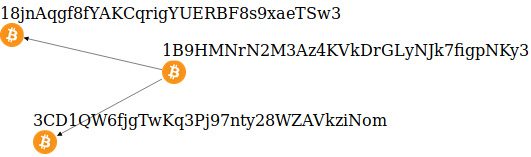
\includegraphics[scale=0.35]{images/exampleWithGraph/naturalAddressGrahScamTx.png}
   \caption{Frammento del grafo naturale degli address descritto dalla transazione con identificativo 82\-a69\-be69e\-00937\-91ab7\-d3803\-69ec\-ffba4f\-1fe08\-27a862\-5ede9\-d89e9\-4776b\-c21.\label{fig:addGrapjNatural}}
   \end{figure}

   Il grafo naturale di address risulta essere troppo superficiale, perché le chiavi pubbliche che fanno parte dello script da cui è ottenuto l'address \say{3CD1\-QW6fjg\-TwKq3Pj\-97nty28W\-ZAVkz\-iNom} potrebbero essere riutilizzate singolarmente all'interno della blockchain di Bitcoin passando inosservate agli algoritmi di analisi;
   \item Il grafo degli address ottenuto con un'analisi degli indirizzi originati da script. A titolo d'esempio, il frammento di grafo illustrato nella Figura \ref{fig:addGrapjNatural} in cui viene condotta un'analisi dello script da cui viene originato l'address \say{3CD1\-QW6fjg\-TwKq3Pj\-97nty28W\-ZAVkz\-iNom} viene illustrato nella Figura \ref{fig:addGraphAnalisis}
   \begin{figure}[H]
   \centering
   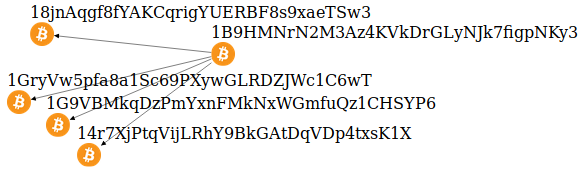
\includegraphics[scale=0.35]{images/exampleWithGraph/decode-address-graph-scam.png}
   \caption{Frammento del grafo degli address ottenuto attraverso un analisi dell'address 3CD1\-QW6fjg\-TwKq3Pj\-97nty28W\-ZAVkz\-iNom.\label{fig:addGraphAnalisis}}
   \end{figure}
   Il grafo di address appena descritto risolve la problematica riguardante le chiavi pubbliche, contenute all'interno dello script, con la conseguenza della perdita del riferimento riguardante l'address originato dallo script, il che aumenta notevolmente il grado di complessità del grafo.\\
   Una possibile soluzione, potrebbe essere quella di utilizzare una rappresentazione attraverso il grafo naturale rappresentato dalla Figura \ref{fig:addGrapjNatural}, con l'aggiunta delle chiavi pubbliche ricavate dallo script come proprietà del nodo, ottenendo la rappresentazione illustrata in Figura \ref{fig:addGrapjNaturalPlus}
   \begin{figure}[H]
   \centering
   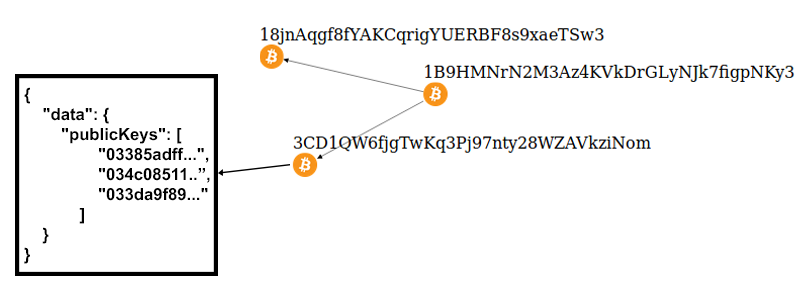
\includegraphics[scale=1.4]{images/exampleWithGraph/naturalAddressGrahScamTx_correcter.png}
   \caption{Frammento del grafo naturale degli address arricchito delle informazioni delle chiavi pubbliche all'interno del nodo.\label{fig:addGrapjNaturalPlus}}
   \end{figure}
 \end{itemize}

 In seguito allo studio di fattibilità sulla creazione del grafo, ci siamo limitati alla costruzione di un grafo semplificato, anche perché oltre alle problematiche descritte abbiamo dovuto affrontare anche le problematiche sulla serializzazione delle transazioni M:N (molti a molti): ogni transazione può contenere, infatti, M transazioni di input e N transazioni di output.\\
 Questa caratteristica riguardante il numero di transazioni può essere risolta utilizzando una rappresentazione a multigrafo degli address.
 In questo documento, proponiamo una soluzione in cui si forza l'utilizzo di un comune grafo, in cui ogni transazione M:N viene serializzata in maniera iterativa: la prima transazione di input viene serializzata con tutte le transazioni di output e così a seguire, per le restanti transazioni di input, ignorando per il momento il problema delle chiavi pubbliche contenute all'interno degli script da cui si originano address.
 Un frammento del grafo rappresentante una transazione M:N è illustrato dalla Figura \ref{fig:iterativeAddTx}

\begin{figure}
\centering
 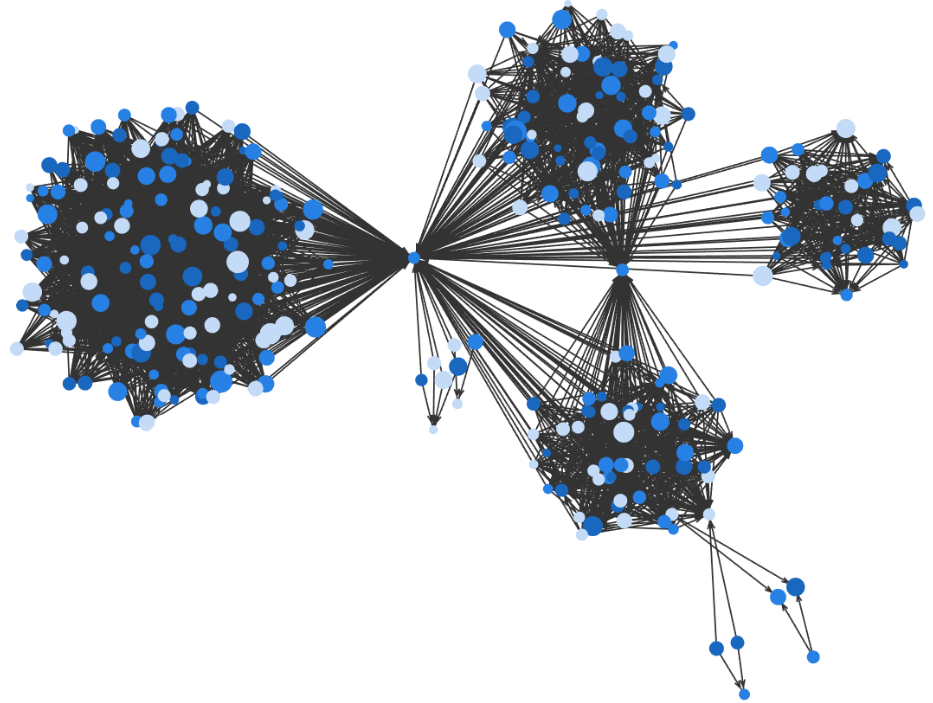
\includegraphics[scale=0.35]{images/demo/iterationTx.png}
 \caption{Frammento del grafo degli address, in cui viene rappresentata una serializzazione iterativa di una transazione M:N.}
 \label{fig:iterativeAddTx}
\end{figure}

 La costruzione del grafo attraverso SpyCBlock avviene grazie all'introduzione del sottomodulo SpyCBlockRPC descritto nella Sezione \ref{sec:spycblockrpc}, il quale si occupa di accedere alle informazioni della transazione precedente tramite l'utilizzo del framework RPC di Bitcoin-core descritto nella Sezione \ref{sec:jsonrpchttp}.
 Il parser inoltre utilizza il framework RPC per decodificare lo script di blocco, da cui si ottiene l'address oppure gli address contenuti al suo interno.\\
 Il framework RPC di Bitcoin-core non essendo adatto all'estrazione completa delle informazioni dalla blockchain di Bitcoin limita le prestazioni del parser durante l'analisi delle informazioni.\\
 Questo problema potrebbe essere risolto estendendo l'implementazione di SpyCBlockRPC ad un implementazione \emph{multi thread} oppure implementando un decompilatore per gli script di Bitcoin; quest'ultima soluzione implica anche l'implementazione di un metodo di memorizzazione per mantenere una cronologia delle transazioni decodificate dal parser.

 Una porzione di grafo degli address viene rappresentata dalla Figura \ref{fig:addressGraph}

\begin{figure}
\centering
 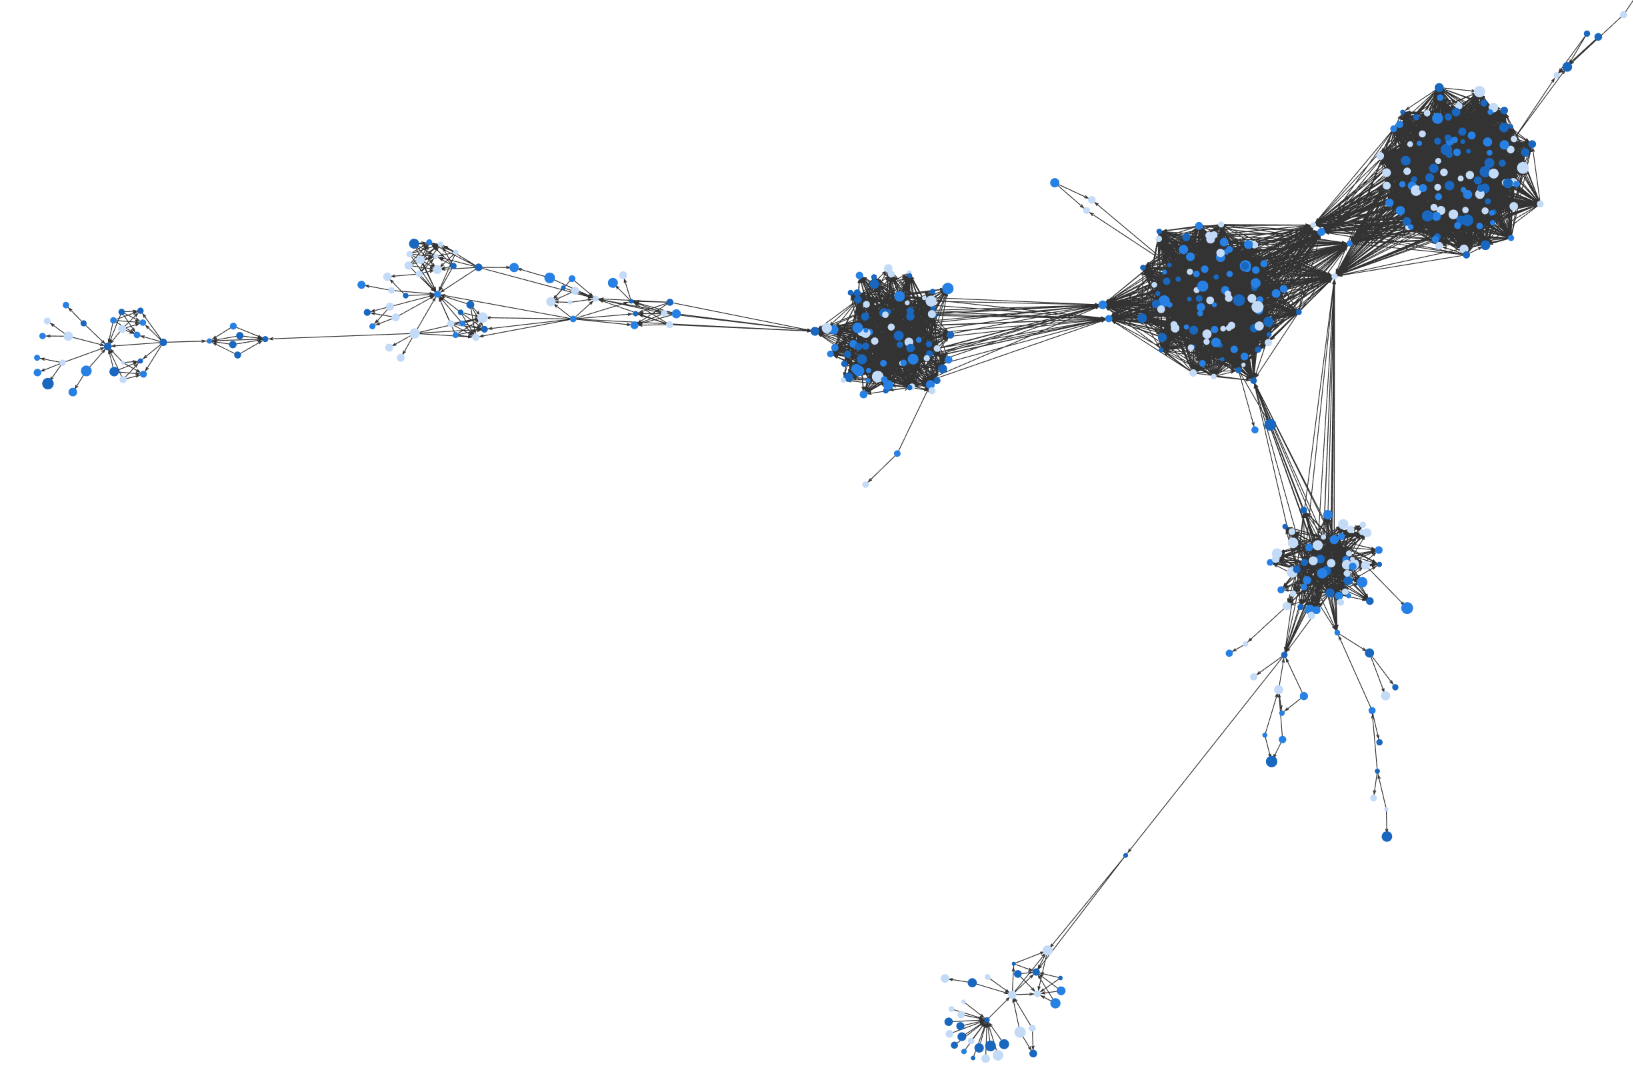
\includegraphics[scale=0.25]{images/demo/address_graph.png}
 \caption{Frammento del grafo degli address estrapolato dalla demo descritta nella Sezione \ref{sec:SpyJSBlock}.}\label{fig:addressGraph}
\end{figure}

\section{Risultati Sperimentali} \label{sec:valutazionesperimentale}

La soluzione proposta si è limitata all'estrazione dei dati dalla blockchain di Bitcoin in modo scalabile con una successiva riconversione dei dati tale da consentire la costruzione di un grafo di transazioni, oltre alla serializzazione completa in JSON della blockchain.\\
Il parser proposto come soluzione oltre a serializzare il grafo di transazioni implementa anche una soluzione sperimentale per la creazione del grafo di address attraverso l'ausilio del framework RPC di Bitcoin descritto nella Sezione \ref{sec:jsonrpchttp}.\\
Nella valutazione sperimentale condotta è stato analizzato il tempo necessario   per la serializzazione in JSON della blockchain e per la serializzazione del grafo di transazioni, ignorando il tempo di serializzazione del grafo di address in quanto fortemente dipendente dal framework RPC.\\
L'analisi viene condotta eseguendo il parser su una CPU \say{Intel Core i7-4790} con 8 Core da 4Ghz l'uno; le prestazioni su \emph{single core} vengono illustrate nella Figura \ref{fig:noparallelbenchmark}, dove sulle ascisse si trova la quantità di dati decodificati dal parser e sulle ordinate si trovano  i minuti necessari per eseguire tale operazione.
\begin{figure}[H]
\centering
 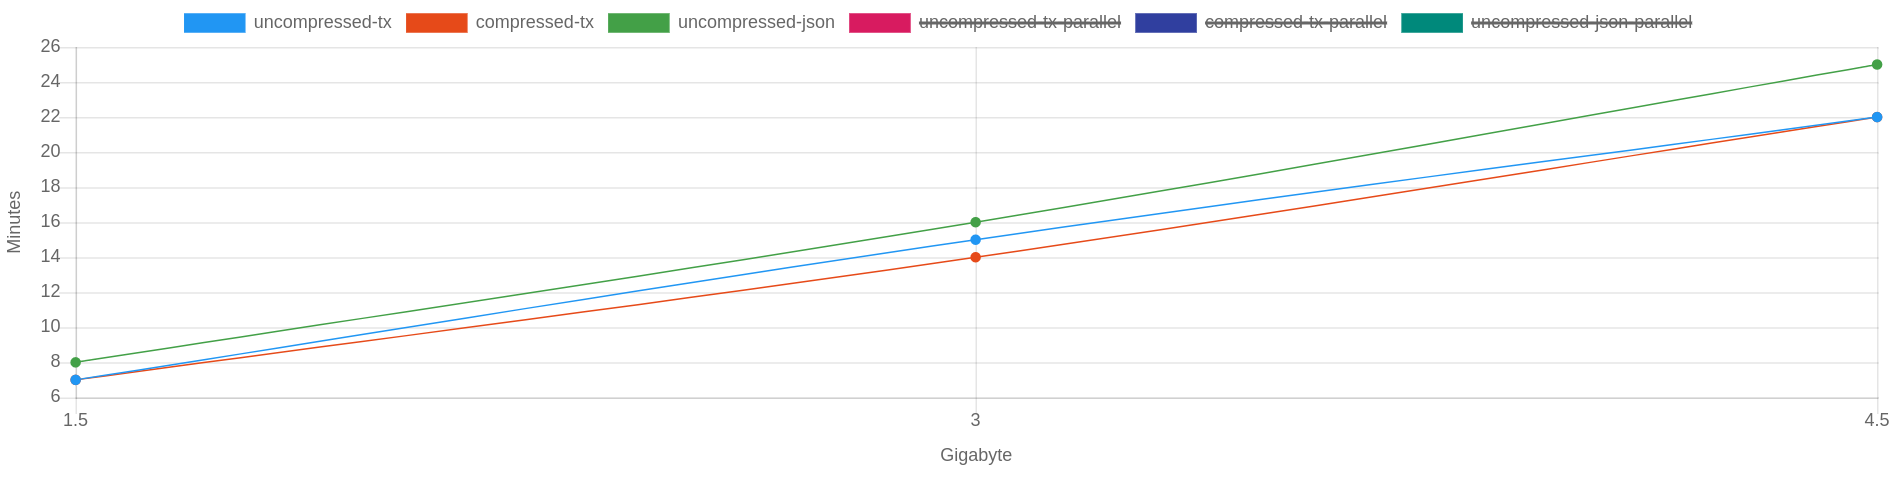
\includegraphics[scale=0.2]{images/demo/no_paralel_benckmark.png}
 \caption{Grafico delle prestazioni del parser su \emph{single core}.}\label{fig:noparallelbenchmark}
\end{figure}

Osservando le prestazioni descritte dalla Figura \ref{fig:noparallelbenchmark} abbiamo notato che la velocità dell'analisi dipende fortemente dal tipo di CPU utilizzata; sulla base di tale  osservazione abbiamo aggiunto la possibilità di eseguire il parser su più processori attraverso la libreria OpenMP descritta nella Sezione \ref{sec:openmp}.\\
Con l'esecuzione parallela del parser abbiamo ottenuto un netto miglioramento delle prestazioni, le quali vengono descritte nella Figura \ref{fig:parallelbenchmark} dove i tempi  per la serializzazione in JSON (linea verde) e per la creazione del grafo di transazioni non compresso (linea viola) sono sovrapposti.\\

\begin{figure*}
	\centering
	\subfigure[][Grafico delle prestazioni del parser eseguito su multiprocessore.]{\label{fig:parallelbenchmark}
		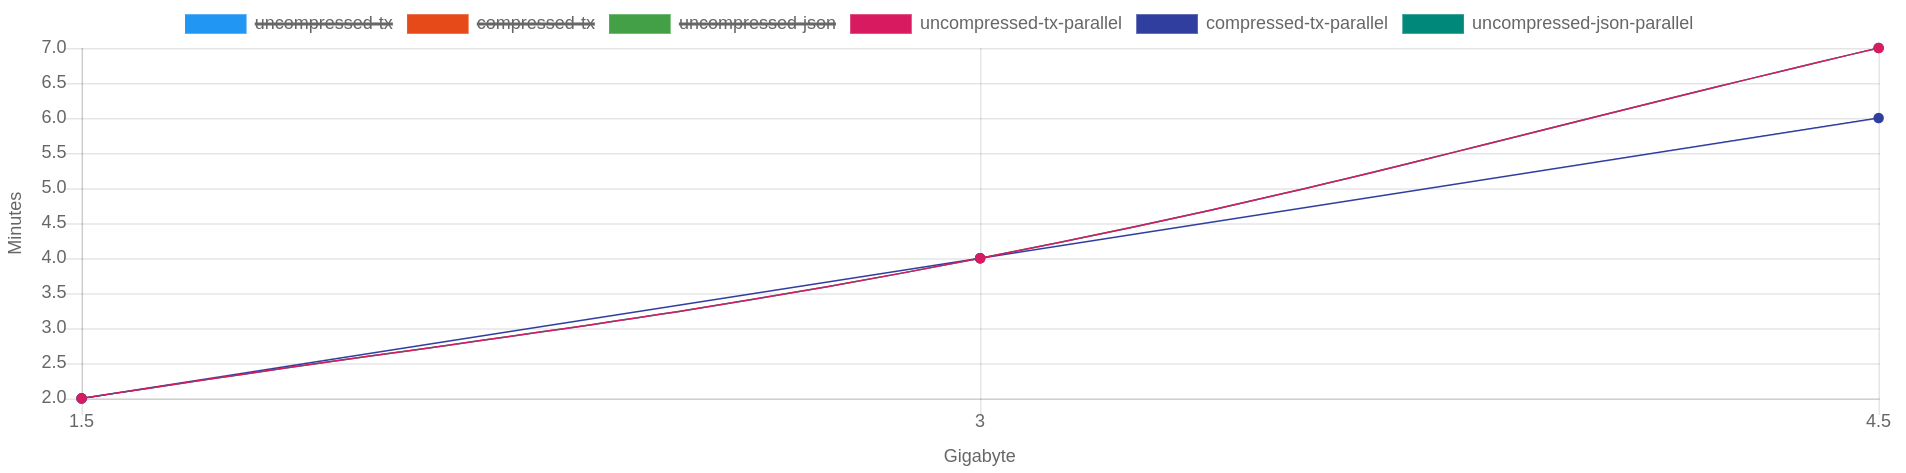
\includegraphics[width=.8\linewidth]{images/demo/parallel_scalability.png}}
	\subfigure[][Confronto tra versione single core e multi-core.]{\label{fig:sovrapposition}
		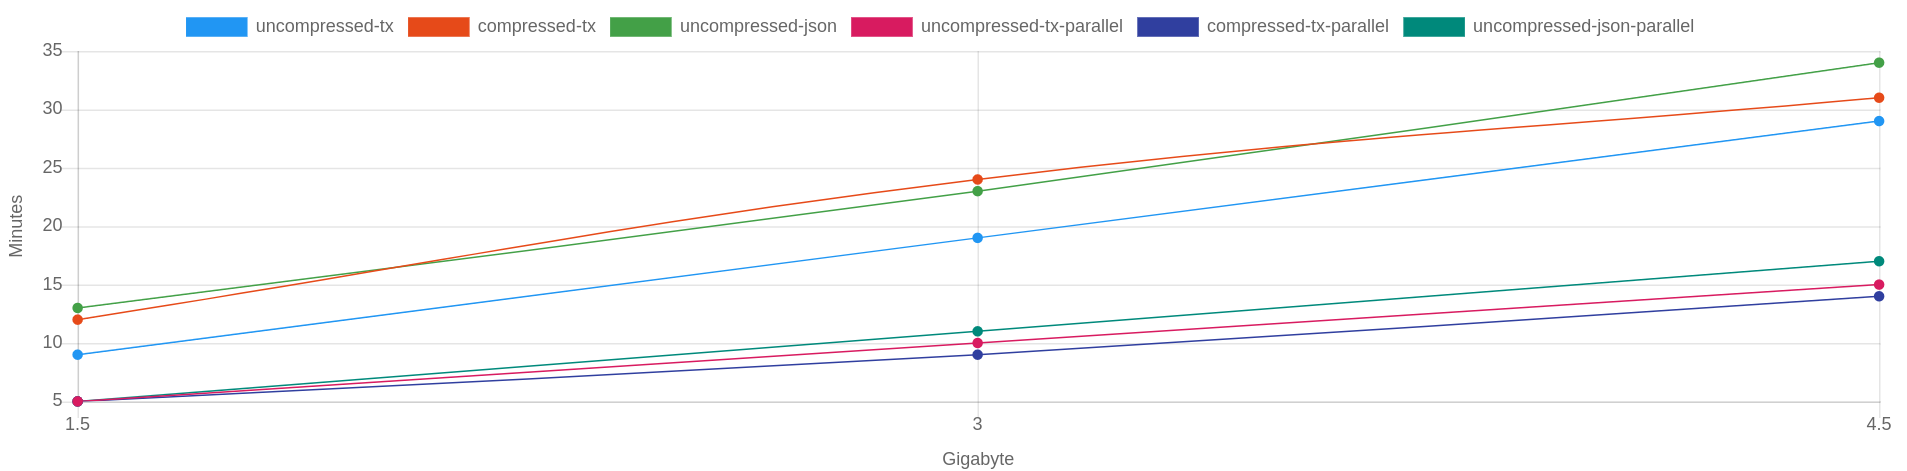
\includegraphics[width=.8\linewidth]{images/demo/sovrapposition_benchmark.png}}
	\caption{Grafici delle prestazioni del parser descritti nel seguente capitolo.}
	\label{fig:analisisScript}
\end{figure*}

Al momento della stesura del documento la versione parallelizzata del parser utilizza tutti i core disponibili dal processore quindi nella nostra valutazione sperimentale, il parser analizza otto file contemporaneamente.\\
La Figura \ref{fig:sovrapposition} descrive il confronto tra l'esecuzione single core e quella parallela.\\
Il parser, attraverso l'esecuzione parallela con la CPU presa in considerazione in questa valutazione sperimentale, esegue l'analisi sull'intera blockchain in 8 ore\footnote{Tali risultati fanno riferimento alla dimensione della blockchain assunta nel novembre del 2019: 604.038 blocchi e 249 GB di spazio totale.}, con un netto miglioramento sulla versione single core che effettua l'analisi sull'intera blockchain in circa 3 giorni.

\section{DEMO} \label{sec:solDemo}

\subsection{AnalyticsPyBlock} \label{sec:AnalyticsPyBlock}

\begin{figure*}
	\centering
	\subfigure[][Grafico che rappresenta gli script più utilizzati all'interno la blockchain di Bitcoin.]{\label{fig:globalAnalisis}
		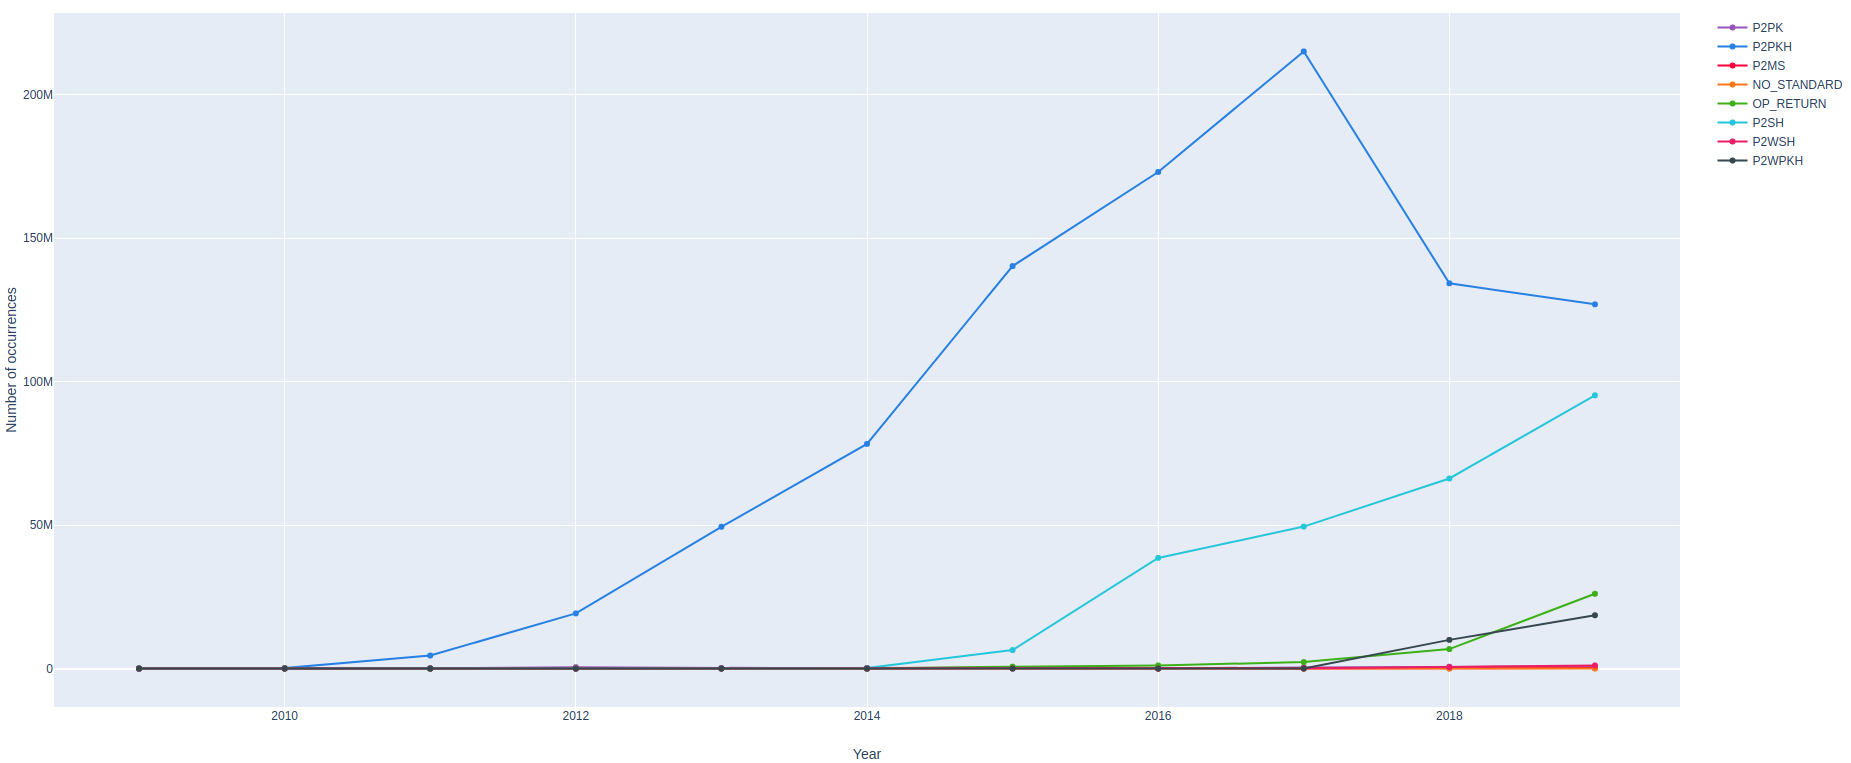
\includegraphics[width=.8\linewidth]{images/demo/analytics/result-global.png}}
	\subfigure[][Grafico che rappresenta l'utilizzo dello script OP\_RETURN per archiviare dati.]{\label{fig:optReturnScript}
		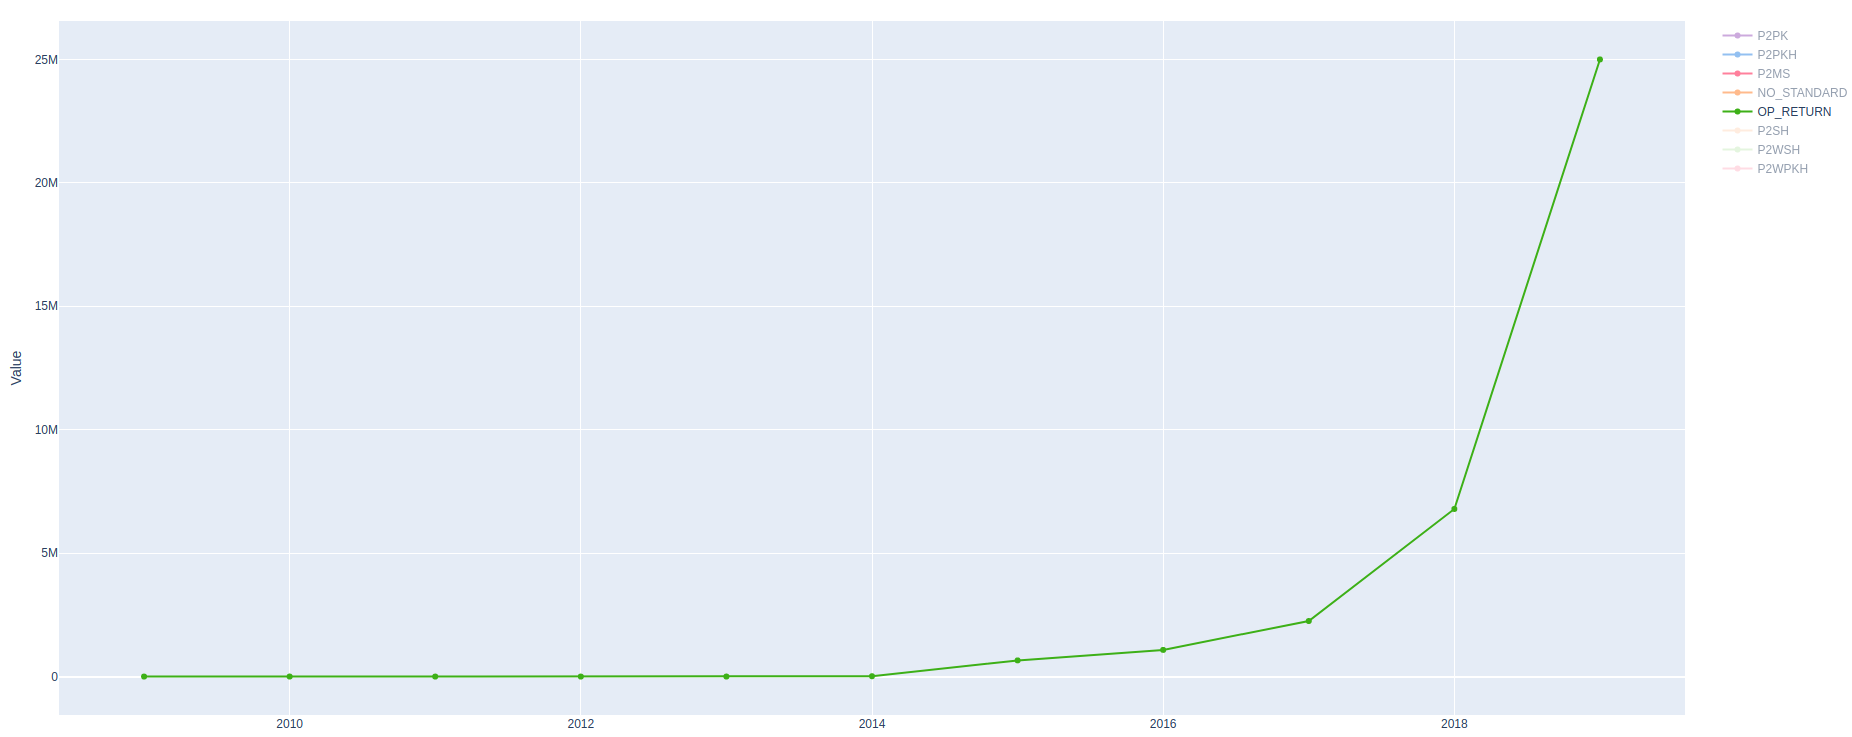
\includegraphics[width=.8\linewidth]{images/demo/analytics/opt_return.png}}
	\caption{Grafici estrapolati dalla demo descritta nel seguente capitolo.}
	\label{fig:analisisScript}
\end{figure*}

Per dimostrare un possibile utilizzo della blockchain di Bitcoin serializzata in JSON è stata sviluppato un semplice strumento di analisi denominato AnalyticsPyBlock, il quale permette anche di sviluppare analisi personalizzate.\\
AnalyticsPyBlock al momento della stesura del documento supporta solo un tipo di analisi, riguardante la tipologia di script utilizzati nel tempo nella rete Bitcoin; il software di analisi viene sviluppato in Python3 e risiede su Github sotto licenza Apache License 2.0.\\
La Figura \ref{fig:analisisScript} illustra il risultato dell'analisi sulle tipologie di script.

%    \begin{figure}
%    \begin{subfigure}{\textwidth}
%      \centering
%      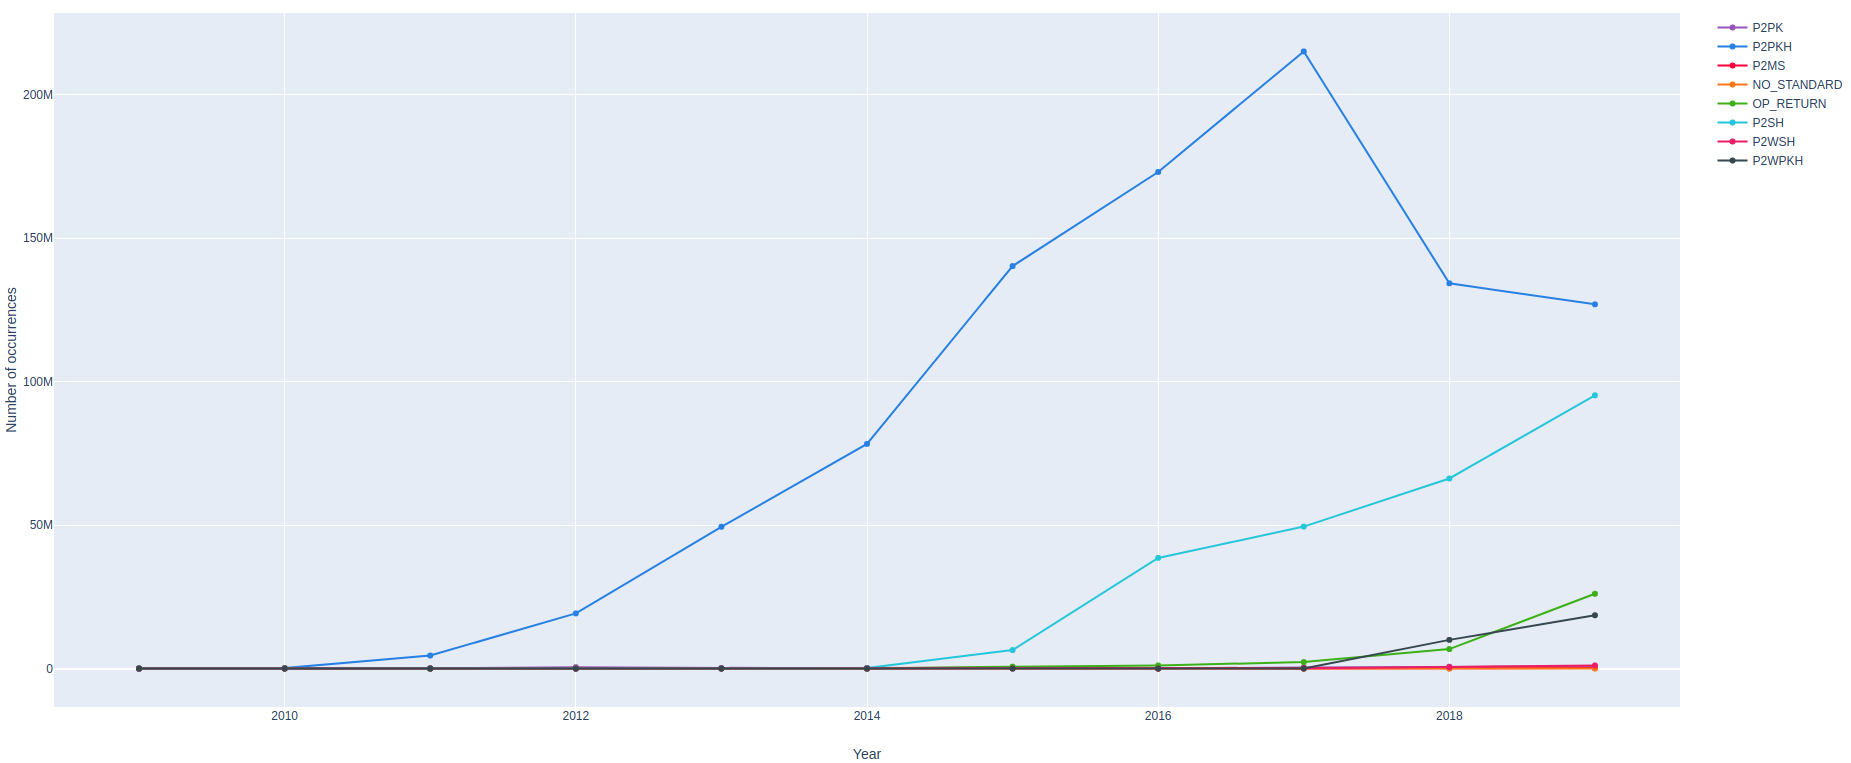
\includegraphics[width=.8\linewidth]{images/demo/analytics/result-global.png}
%      \caption{1a. Grafico che rappresenta gli script più utilizzati all'interno la blockchain di Bitcoin.}
%      \label{fig:globalAnalisis}
%    \end{subfigure}%
%    \begin{subfigure}{\textwidth}
%      \centering
%      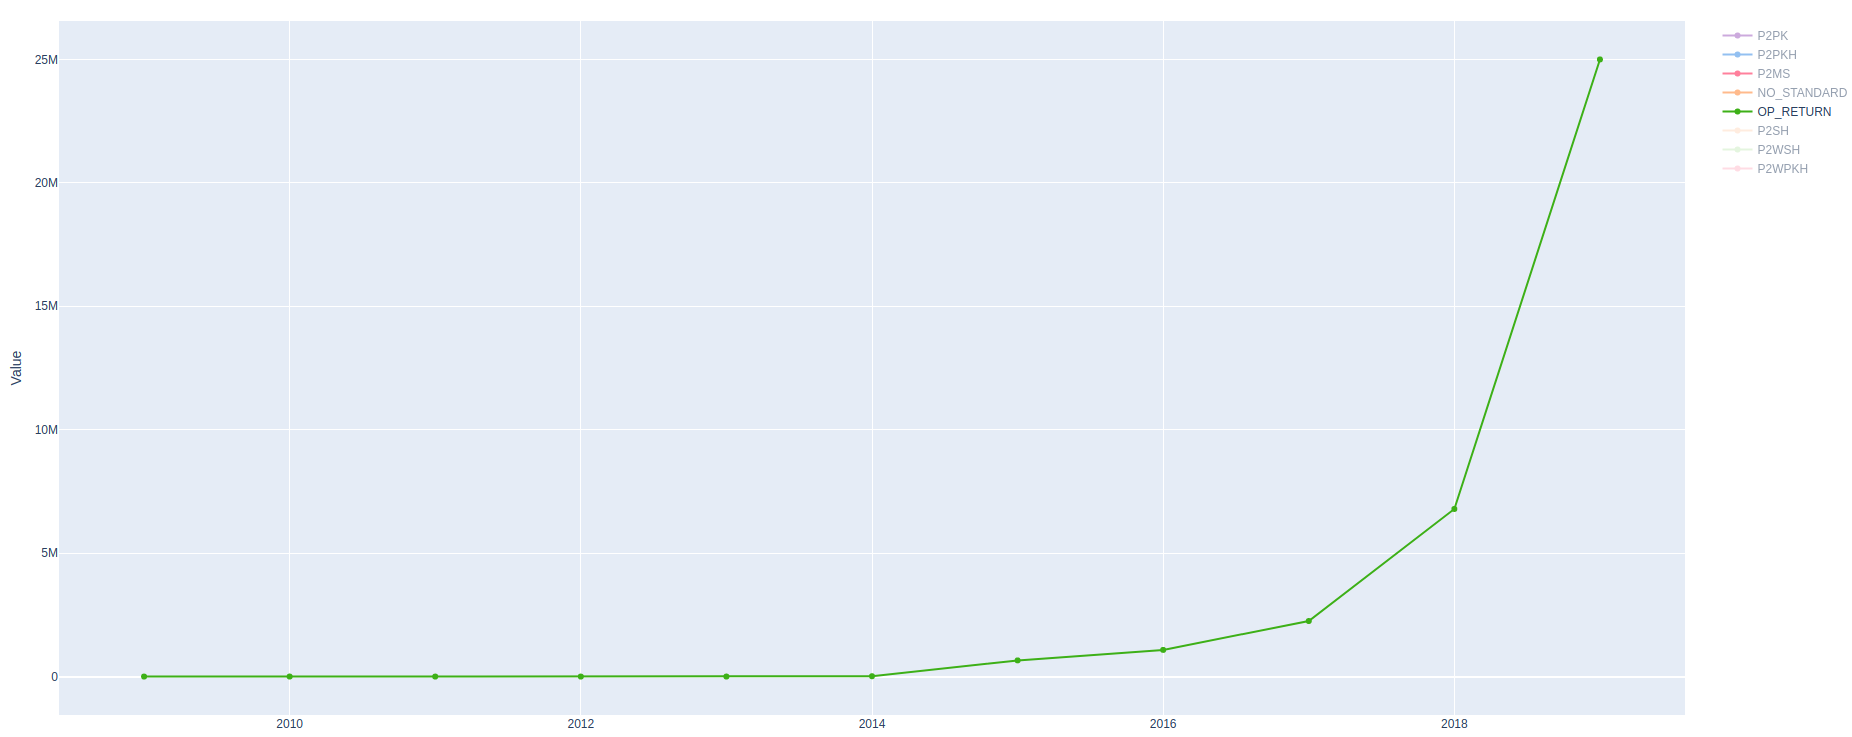
\includegraphics[width=.8\linewidth]{images/demo/analytics/opt_return.png}
%      \caption{1b.  Grafico che rappresenta l'utilizzo dello script OP\_RETURN per archiviare dati.}
%      \label{fig:optReturnScript}
%    \end{subfigure}
%    \caption{Grafici estrapolati dalla demo descritta nel segunte capitolo.}
%    \label{fig:analisisScript}
%    \end{figure}

La Figura \ref{fig:globalAnalisis} mostra gli script maggiormente utilizzati, che risultano essere P2PKH e  P2SH; inoltre la Figura \ref{fig:optReturnScript} mostra l'utilizzo della blockchain di Bitcoin per l'archiviazione di dati. Questa informazione è molto utile ai fini della costruzione del grafo perché attraverso una futura operazione di \emph{data cleaning} si possono eliminare tutte le informazioni che riguardano l'archiviazione di dati attraverso l'operatore OP\_RETURN.\\
La strumento impiega meno di 8 ore per analizzare i file JSON serializzati da SpyCBlock; anche tale tool potrebbe essere migrato ad un'implementazione multiprocessore con cui si può migliorare la velocità di analisi.

\subsection{SpyJSBlock} \label{sec:SpyJSBlock}

Per visualizzare i grafi serializzati da SpyCBlock abbiamo sviluppato un'applicazione web che fa uso delle librerie appartenenti alla famiglia ngraph descritte nella Sezione \ref{sec:ngraph}, con cui siamo riusciti ad ottenere una visualizzazione di una piccola parte dei grafi serializzati da SpyCBlock.\\
Attraverso la possibilità di visualizzare i grafi, siamo riusciti ad eseguire tutte le analisi discusse in questo documento; inoltre con l'utilizzo del modulo ngraph.louvain abbiamo condotto un'analisi minimale sul grafo degli address scomponendo quest'ultimo in comunità, anche se l'applicazione di tale algoritmo soffre delle problematiche descritte nella Sezione \ref{sec:solGraphAddress}.\\
L'applicativo web viene sviluppato utilizzando JavaScript senza l'ausilio di framework; una possibile evoluzione di questo applicativo potrebbe essere la migrazione ad un framework come React \cite{vis:react}.\\
Lo strumento software possiede due diverse implementazioni per via delle diverse problematiche riguardanti le librerie ngraph descritte nella Sezione \ref{sec:ngraph}; gli applicativi risiedono su Github sotto licenza Creative Commons 4.0 e vengono denominati SpyJSBlock \cite{vis:SpyJSBlock} e SpyJSBlock-NGraph \cite{vis:SpyJSBlock-Ngraph}.
Le principali differenze tra gli strumenti software sono:
\begin{itemize}
  \item SpyJSBlock è una prima implementazione dell'applicativo web che fa uso della libreria VivagraphJS descritta nella Sezione \ref{sec:ngraph}; a causa  della difficoltà nel personalizzare il rendering tramite WebGL, non viene eseguita nessuna personalizzazione tranne che l'aggiunta della possibilità di esplorare i nodi del grafo attraverso eventi di click che offrono la possibilità di ricercare l'id della transazione oppure l'address attraverso un'explorer come Explora \cite{blockstream:esplora}.\\
  Non utilizzando nessuna particolare personalizzazione il rendering risulta essere molto veloce, riuscendo a visualizzare una porzione di grafo abbastanza grande, ma risulta essere difficoltoso cambiare la modalità di rendering oppure applicare algoritmi di analisi sul grafo.\\
  Un frammento di grafo visualizzato attraverso SpyJSBlock viene illustrato attraverso la Figura \ref{fig:vivagraphSpyJSBlock}.

  \begin{figure}
  \centering
   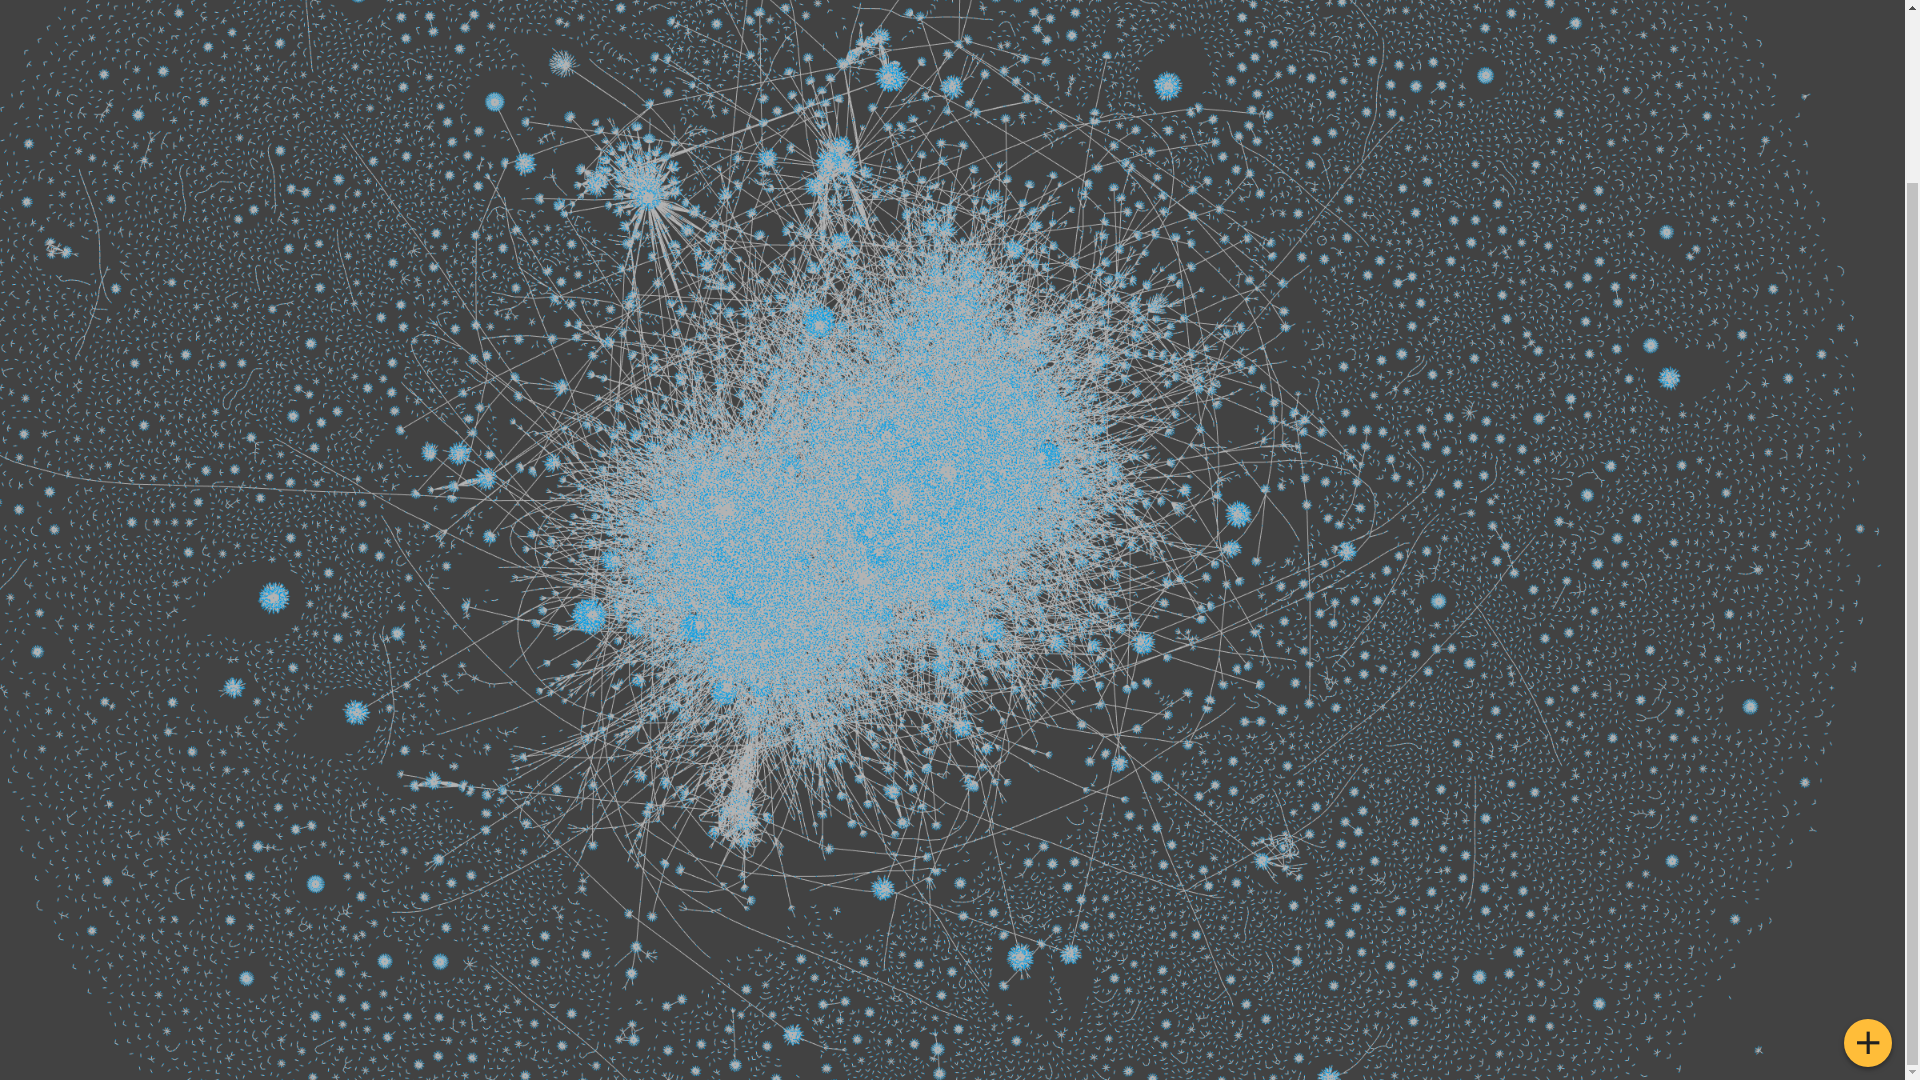
\includegraphics[scale=0.2]{images/demo/vivagraph.png}
   \caption{Frammento del grafo visualizzato attraverso l'applicativo SpyJSBlock.}\label{fig:vivagraphSpyJSBlock}
  \end{figure}

  Per personalizzare il rendering ed avere più controllo sulla visualizzazione del grafo abbiamo sviluppato un'alternativa utilizzando le librerie della famiglia ngraph.
  \item SpyJSBlock-NGraph è un raffinamento dello strumento SpyJSBlock, dove vengono utilizzati i moduli della famiglia ngraph per il rendering dei grafi, con cui si riesce ad ottenere un miglioramento nella qualità del rendering, a discapito però delle performance, con la conseguenza di renderizzare una porzione più piccola del grafo.
  Viene utilizzato il modulo ngraph.pixel per il rendering in 3D del grafo delle transazioni, in cui viene implementata anche la possibilità di ricercare l'id della transazione attraverso l'explorer Explora, La Figura \ref{fig:ngraph.pixel3d} illustra un frammento del grafo delle transazioni.

  Per il rendering del grafo degli address invece viene utilizzato il modulo ngraph.pixi con cui si riesce ad ottenere una visualizzazione 2D di un grafo diretto, di cui la Figura \ref{fig:pixiaddress} illustra un esempio.
  Inoltre, sul grafo degli address viene applicato un algoritmo di ricerca delle comunità attraverso il modulo ngraph.louvain descritto nella Sezione \ref{sec:ngraph}.\\
  Dopo l'applicazione dell'algoritmo, le comunità di nodi vengono dipinte con colori diversi, semplificando l'individuazione di queste ultime all'interno del grafo.\
  La Figura \ref{fig:pixilouvianaddress} illustra una scomposizione in comunità del grafo degli address.

  \begin{figure*}
  	\centering
    \subfigure[][Frammento del grafo delle transazioni visualizzato attraverso l'applicativo SpyJSBlock-NGraph.]{\label{fig:ngraph.pixel3d}
  		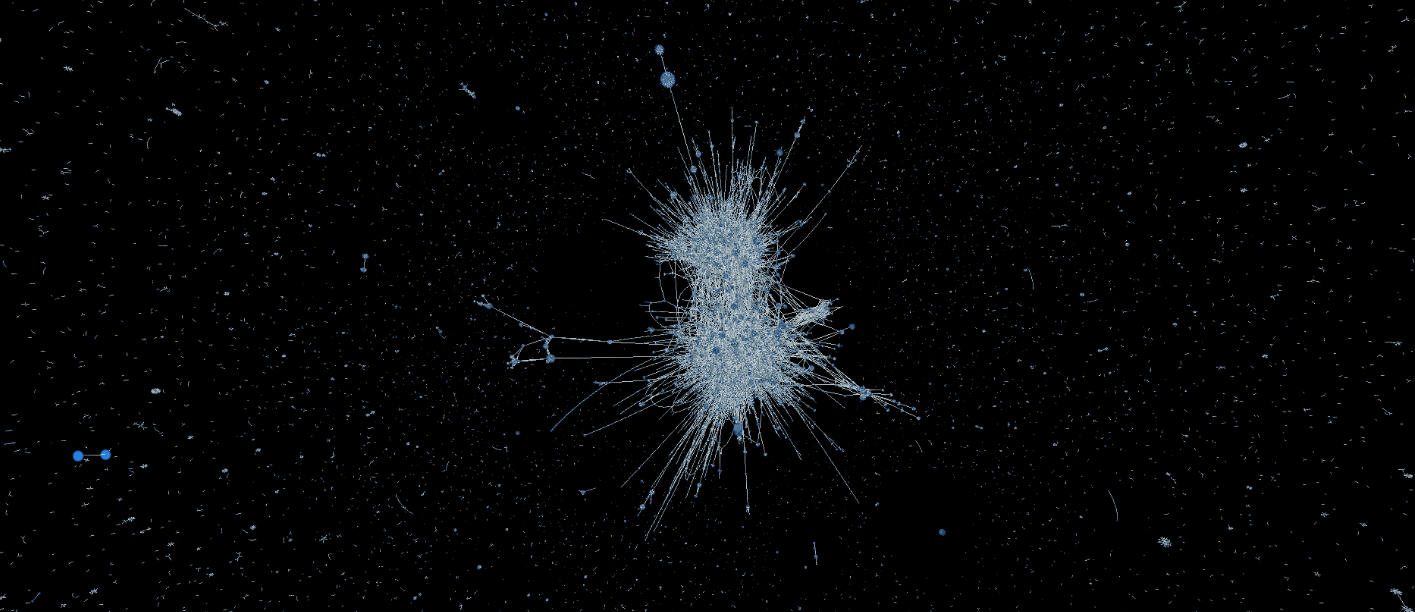
\includegraphics[width=.75\linewidth,scale=0.75]{images/demo/3D_tx.png}}
  	\subfigure[][Grafo degli address visualizzato attraverso il modulo ngraph.pixi \cite{vis:ngraph.pixi}.]{\label{fig:pixiaddress}
  		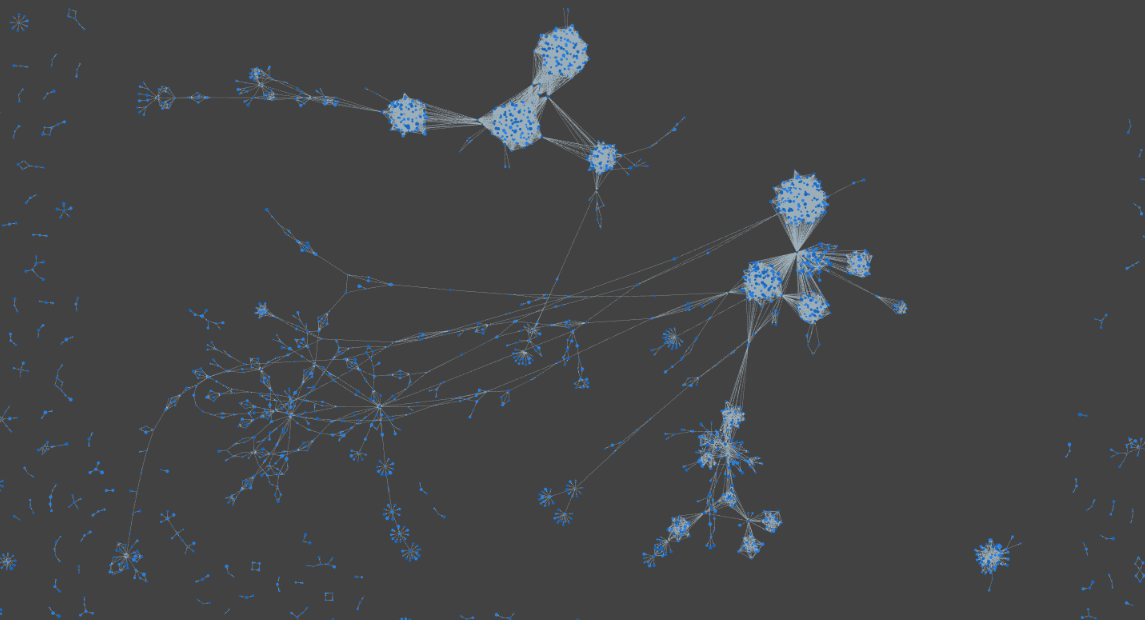
\includegraphics[width=.75\linewidth]{images/demo/ngraphpixi.png}}
  	\subfigure[][Grafo degli address scomposto in comunità attraverso l'utilizzo del modulo ngraph.louvain \cite{ngraph.louvain}]{\label{fig:pixilouvianaddress}
  		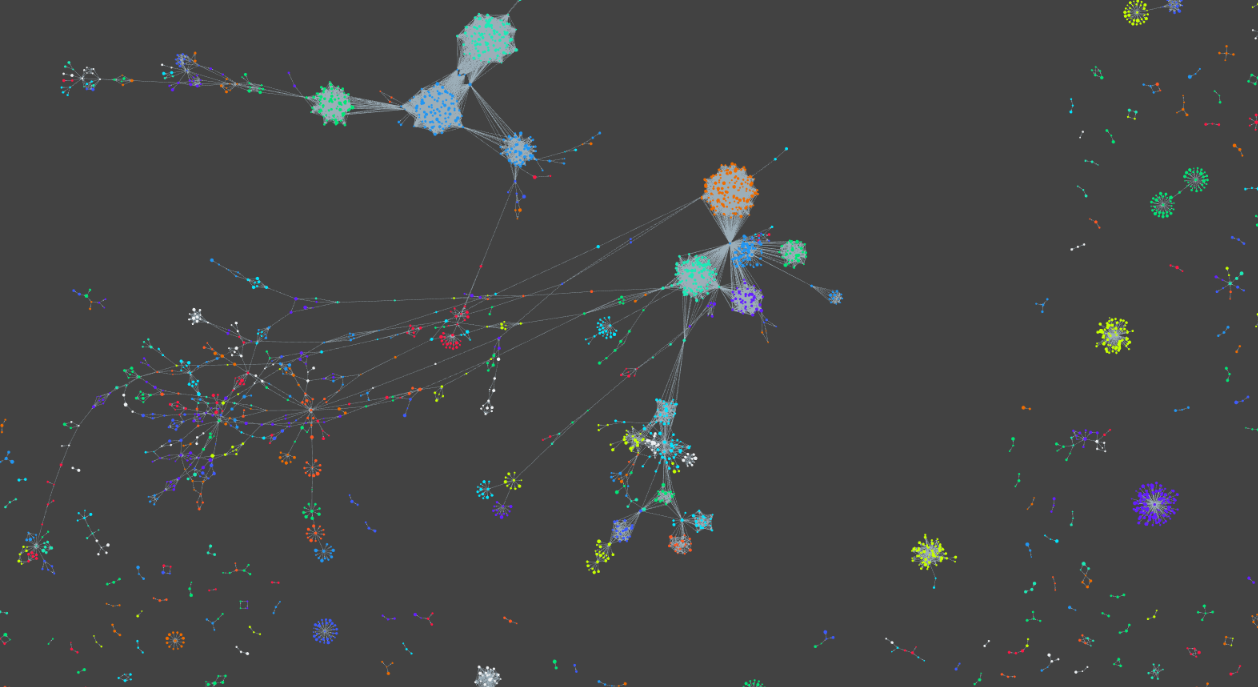
\includegraphics[width=.75\linewidth]{images/demo/ngraphlouvian.png}}
  	\caption{Frammenti  dei grafi estrapolati dagli applicativi descritti nel seguente capitolo.}
  	\label{fig:ngraphvis}
  \end{figure*}

\end{itemize}
